\documentclass{article}
\usepackage[top=1in, bottom=1in, left=1.25in, right=1.25in]{geometry}
\usepackage{amsmath,amssymb}
\usepackage{xcolor}
\usepackage{graphicx}
\setlength{\parindent}{0pt}
\usepackage[utf8]{inputenc}
 
\usepackage{listings}
\usepackage{color}
 
\definecolor{codegreen}{rgb}{0,0.6,0}
\definecolor{codegray}{rgb}{0.5,0.5,0.5}
\definecolor{codepurple}{rgb}{0.58,0,0.82}
\definecolor{backcolour}{rgb}{0.95,0.95,0.92}
 
\lstdefinestyle{mystyle}{
    backgroundcolor=\color{backcolour},   
    commentstyle=\color{codegreen},
    keywordstyle=\color{magenta},
    numberstyle=\tiny\color{codegray},
    stringstyle=\color{codepurple},
    basicstyle=\footnotesize,
    breakatwhitespace=false,         
    breaklines=true,                 
    captionpos=b,                    
    keepspaces=true,                 
    numbers=left,                    
    numbersep=5pt,                  
    showspaces=false,                
    showstringspaces=false,
    showtabs=false,                  
    tabsize=2
}
 
\lstset{style=mystyle}

\title{ Bios/CS 534 Project 1}
\author{Chenxi Cai}
\begin{document}
\lstset{numbers=left, numberstyle=\small, keywordstyle=\color{blue!70}, commentstyle=\color{red!50!green!50!blue!50}, frame=shadowbox, rulesepcolor=\color{red!20!green!20!blue!20},escapeinside=``, xleftmargin=2em,xrightmargin=2em, aboveskip=1em}
\maketitle
\section{Problem 1}
Class Y = 0:

\textbf{mean vector:}
\begin{equation}
		\begin{bmatrix}
1.06242164  & 1.61910524
			\end{bmatrix}
			\end{equation}
\textbf{covariance matrix:}
		\begin{equation}
		\begin{bmatrix}
4.79170095 & 0.90180838 \\
0.90180838 & 1.2945715 
			\end{bmatrix}
			\end{equation}
Class Y = 1:

\textbf{mean vector:}
\begin{equation}
		\begin{bmatrix}
1.13915258 &  -1.18380439
			\end{bmatrix}
			\end{equation}
\textbf{covariance matrix:}
		\begin{equation}
		\begin{bmatrix}
0.7560476 &  -0.5093068 \\
-0.5093068 &  3.19387164
			\end{bmatrix}
			\end{equation}

	\subsection{Equal prior case}
Classification error rate on the testing data is
			 \begin{equation}
				0.057692
				\end{equation}
Scatter plots with boundary  of the training data is shown as Figure \ref{fig:equal_prior}.

The s in Class y = 0 and y = 1 is red "o" and  blue "x", separately.
\begin{figure}[!hbp]
    		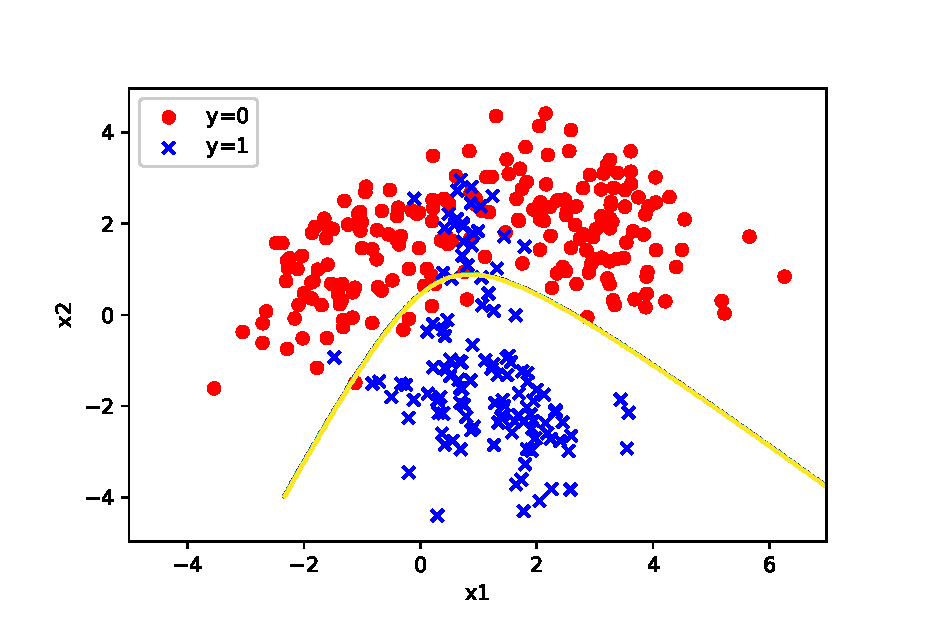
\includegraphics[width=5 in]{Equal_prior.eps}
		\centering
		\caption{Scatter plots with boundary of equal prior}
		\label{fig:equal_prior}
    		\end{figure}

\subsection{Prior calculated from the data case}
Classification error rate on the testing data is
			 \begin{equation}
				0.057692
				\end{equation}
Scatter plots with boundary  of the training data is shown as Figure \ref{fig:data_prior}
\begin{figure}[!hbp]
    		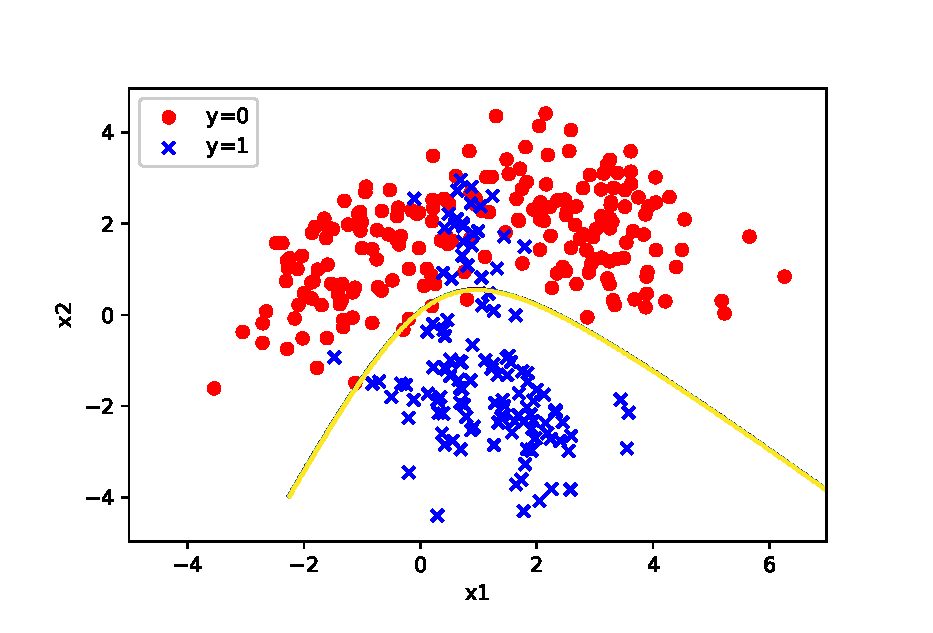
\includegraphics[width=5 in]{Prior_calculated_from_the_data.eps}
		\centering
		\caption{Scatter plots with boundary  of prior calculated from the data}
		\label{fig:data_prior}
    		\end{figure}
\newpage
\section{Problem 2}
	\subsection{Bandwidth=10}
Classification error rate on the testing data is
			 \begin{equation}
				0.184615 
				\end{equation}
Scatter plots of the testing data is shown as Figure \ref{fig:d=10}.

Right points are black and misclassified points are red. The shape of points in Class y = 0 and y = 1 is "o" and "x", separately.
\begin{figure}[!hbp]
    		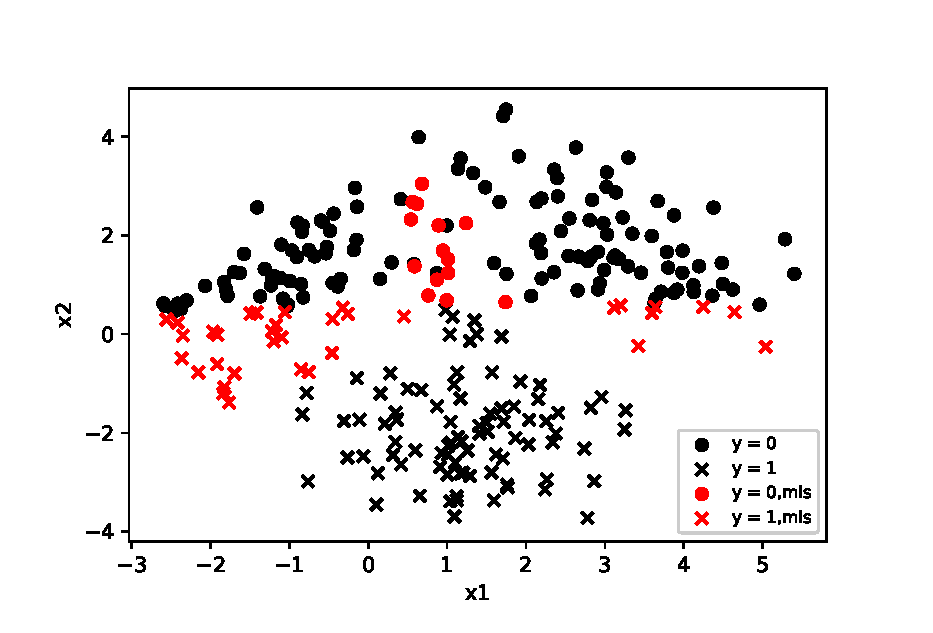
\includegraphics[width=5 in]{bandwidth10.eps}
		\centering
		\caption{Scatter plots of bandwidth=10}
		\label{fig:d=10}
    		\end{figure}
	\subsection{Bandwidth=1}
Classification error rate on the testing data is
			 \begin{equation}
				0.053846
				\end{equation}
Scatter plots of the testing data is shown as Figure \ref{fig:d=1}. 
\begin{figure}[!hbp]
    		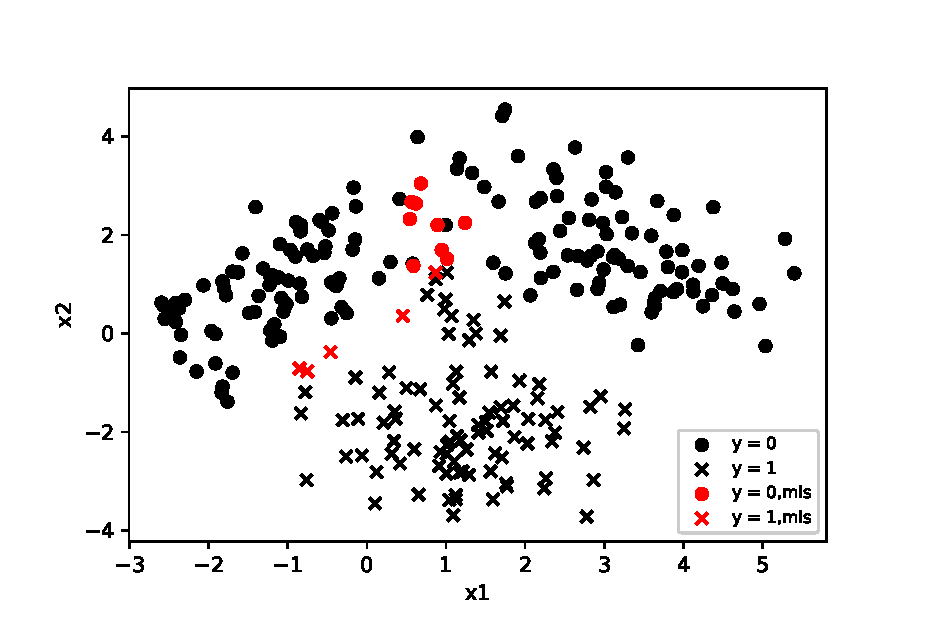
\includegraphics[width=5 in]{bandwidth1.eps}
		\centering
		\caption{Scatter plots of bandwidth=1}
		\label{fig:d=1}
    		\end{figure}
\subsection{Bandwidth=0.1}
Classification error rate on the testing data is
			 \begin{equation}
				0.038462
				\end{equation}
Scatter plots of the training data is shown as Figure \ref{fig:d=0.1}.
\begin{figure}[!hbp]
    		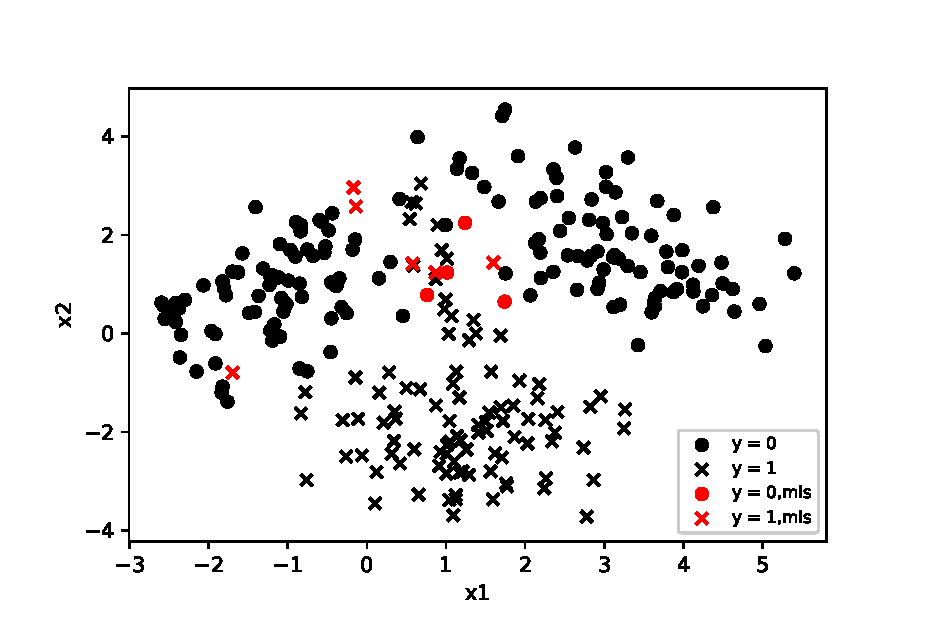
\includegraphics[width=5 in]{bandwidth0.eps}
		\centering
		\caption{Scatter plots of bandwidth=0.1}
		\label{fig:d=0.1}
    		\end{figure}

\newpage
\section{Problem 3}
	\subsection{K=1}
	sensitivity = 0.920000,
	specificity=0.975000, 
	false discovery rate=0.041667 

Scatter plots of the testing data is shown as Figure \ref{fig:K=1}.Right points are black and misclassified points are red. The shape of points in Class y = 0 and y = 1 is "o" and "x", separately.
\begin{figure}[h]
    		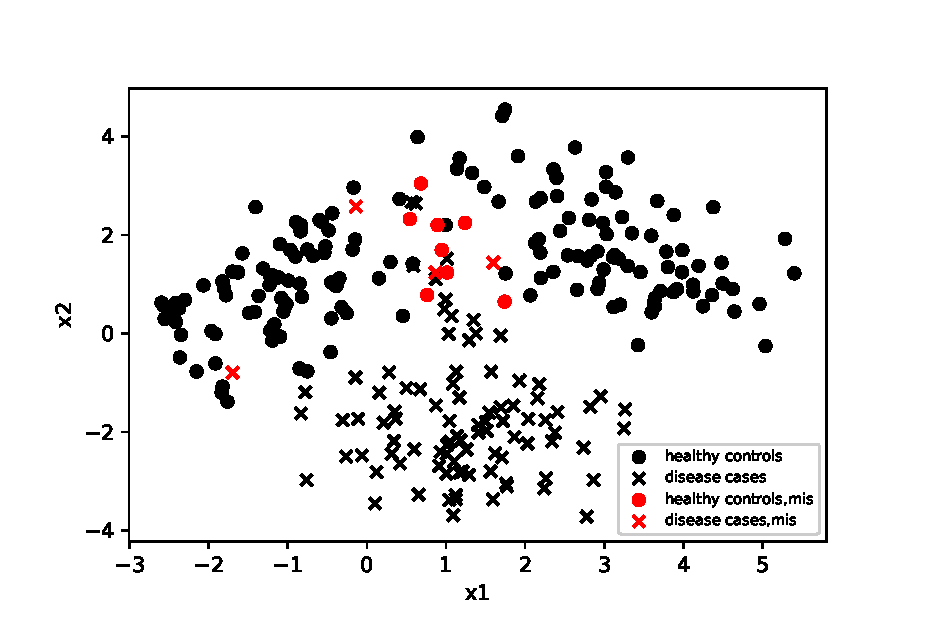
\includegraphics[width=5 in]{k1.eps}
		\centering
		\caption{Scatter plots of K=1}
		\label{fig:K=1}
    		\end{figure}	
	
	\subsection{K=5}
	sensitivity = 0.960000,
	specificity=0.981250, 
	false discovery rate=0.030303 

Scatter plots of the testing data is shown as Figure \ref{fig:K=5}.
\begin{figure}[h]
    		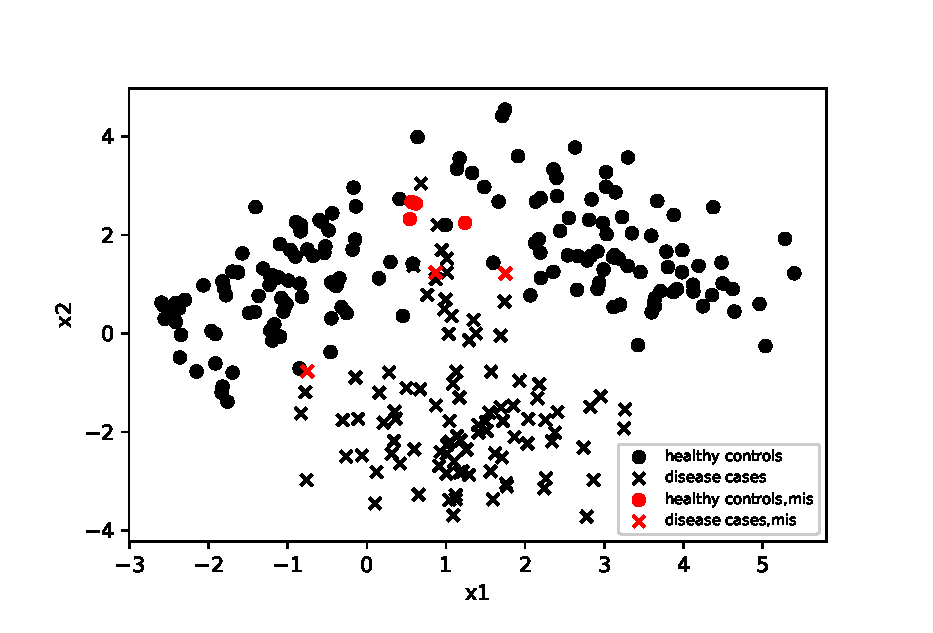
\includegraphics[width=5 in]{k5.eps}
		\centering
		\caption{Scatter plots of K=5}
		\label{fig:K=5}
    		\end{figure}	

	\subsection{K=10}
	sensitivity = 0.950000,
	specificity=0.975000, 
	false discovery rate=0.040404

Scatter plots of the testing data is shown as Figure \ref{fig:K=10}.
\begin{figure}[!h]
    		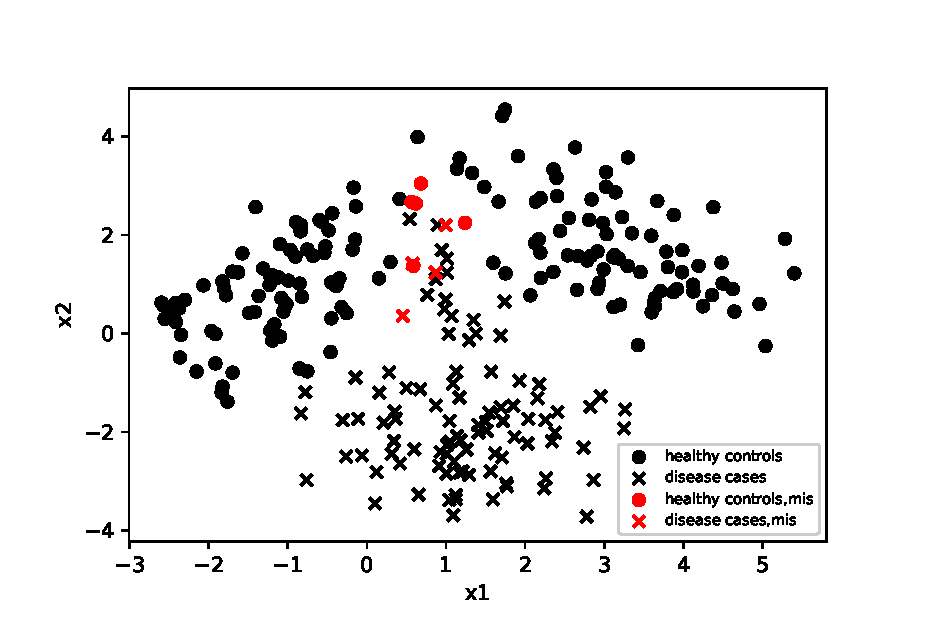
\includegraphics[width=5 in]{k10.eps}
		\centering
		\caption{Scatter plots of K=10}
		\label{fig:K=10}
    		\end{figure}
		
\newpage
\textbf{Python codes of problem1:}
\lstinputlisting[language=Python]{Proj1.1.py}

\textbf{Python codes of problem2:}
\lstinputlisting[language=Python]{Proj1.2.py}

\textbf{Python codes of problem3:}
\lstinputlisting[language=Python]{Proj1.3.py}




\end{document}